% !TeX root = ../main-presentation.tex
\section{Graph rewriting}

\begin{frame}
    \frametitle{Making it combinatorial}

    \LARGE
    \centering
    \scalebox{4}{\textbf{Graph}}

    \scalebox{4}{\textbf{rewriting}}

\end{frame}

\begin{frame}
    \frametitle{Making it combinatorial}

    \centering

    \await

    \dsptikzfig{circuits/productivity/mealy-form}
    \Large
    \await
    \(\Rightarrow\)
    \raisebox{-2em}{
\includegraphics[scale=0.5]{crash}}

    \await

    \vspace{1.5em}

    It is \alert{hard} for computers to work with string diagrams...

    \await

    ...but computers \alert{love} graphs!

\end{frame}

\begin{frame}
    \frametitle{A hyper kind of graph}

    \centering

    \dsptikzfig{graphs/example-trace-cospan}

    \vspace{1em}

    \await
    \Large

    There are correspondences between \alert{certain classes of hypergraphs} and
    \alert{circuit string diagrams}.

    \await
    \normalsize
    \vspace{1em}

    \dsptikzfig{graphs/example-trace-term}

\end{frame}

\begin{frame}
    \frametitle{Using the correspondence}

    \centering
    \Large

    \begin{tikzcd}[ampersand replacement=\&]
        |[visible on=<\iftoggle{static}{1}{1-}>]|\text{Circuit string diagram}
        \arrow[visible on=<\iftoggle{static}{1}{2-}>]{r}
        \arrow[visible on=<\iftoggle{static}{1}{5-}>, equals]{d}
        \&
        |[visible on=<\iftoggle{static}{1}{2-}>]|\text{Hypergraph representation}
        \arrow[visible on=<\iftoggle{static}{1}{3-}>]{d}{\text{\alert{Graph rewrite}}}
        \\
        |[visible on=<\iftoggle{static}{1}{4-}>]|\text{New circuit string diagram}
        \&
        |[visible on=<\iftoggle{static}{1}{3-}>]|\text{Rewritten hypergraph}
        \arrow[visible on=<\iftoggle{static}{1}{4-}>]{l}
    \end{tikzcd}

\end{frame}

\begin{frame}
    \frametitle{Implementing it all}

    \centering
    \Large

    The rewriting framework has been \emph{implemented} in a
    \alert{hardware description language}.

    \begin{center}
        
\includegraphics[width=0.2\textwidth]{huawei}
    \end{center}

    \await

    \small
    (the language is still in development)

    \await

    \scriptsize
    (so I've been warned not to accidentally announce anything)

    \await

    \scalebox{0.75}{
        (also they changed everything so I can't actually compile it at the moment)
    }

\end{frame}

\begin{frame}
    \frametitle{I can still show you something}

    Create a circuit...

    \svg{0}{0.5}{acc}

\end{frame}
\begin{frame}
    \frametitle{I can still show you something}

    The evaluator converts it into \alert{Mealy form}...

    \svg{0}{0.25}{eval-0}

\end{frame}
\begin{frame}
    \frametitle{I can still show you something}

    ...and then evaluates an input.

    \svg{0}{0.2}{after-1}
    \raisebox{5em}{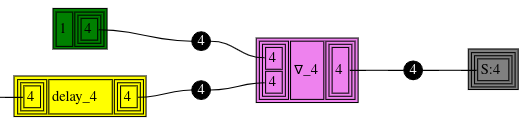
\includegraphics[scale=1.5]{output-1}}

\end{frame}